%!TEX root = ../Thesis.tex
\chapter{Introduction to tools of supervised machine learning}

\section{Supervised machine learning to predict and to learn}
Supervised machine learning is either regression, classification or probability estimation models built on labeled data. Regression is to predict scalars (numbers), classification to predict class membership or lastly to rather predict a probability distribute across class. The direct motive of supervised modeling is to predict a certain target information of a given object, that is otherwise expensive/tedious to measure, or only reveal it self in the future, or the measuring is invasive and will destroy the object of interest. The target is predicted by learning a simple or perhaps complex relationship between easy accessible feature information and the target from a labeled training data set. When a useful relationship has been established with a model, target predictions can be made for a unlabeled data set without the target information. A indirect motive of supervised machine learning, is to elucidate the relationship between features and target. One example of an indirect motive, is when modeling the contraceptive method choice reference data set \cite{welling2016forest,lichman2013uci}. Here, +1000 Indonesian married women had answered a questioner on contraception and socio-economic status. To build a model to accurately predict contraception method choice based on 10 questions on socio-economic status was never the actual motive, as it has little practical use to ask 10 questions to only estimate one answer. Why not just ask the right question once? However, the structure of an accurately predicting model can be a useful empiric proposal for a general relationship in society. Scientificly, the next step is then to form a testable causal link theory based on the observed relationship.

\begin{figure}[!htbp]
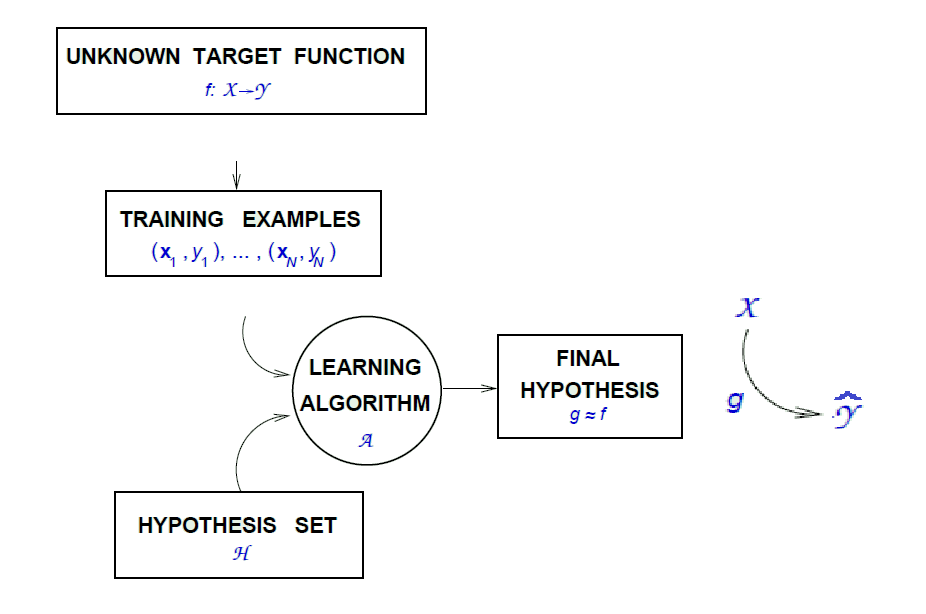
\includegraphics[width=\textwidth,height=\textheight,keepaspectratio]{graphics/sketchMLmapping.png}
\caption{A supervised model learn a relationship between observed features and targets and produce predictions. In order to predict most accurately a robust model with a low prediction error is sought for. One can also use supervised modeling to explore the possible relationship between features and targets, here the question is what is the structure of models providing accurate and robust predictions?} This diagram have been copied from course material from Caltech \cite{Mostafa13learning}.
\label{modelPreditExplain}
\end{figure}

A typical labeled data set, is organized as a data table with one column with desirable target information and a series of columns with feature information. Every row is an independent observation of one target and features. A practical example is the public abalone data set. Here, a marine biologist may be interested in estimating the age of abalones (shellfish). However, determining age is tedious and requires to sacrifice each specimen to study the broken shell under a microscope after chemical staining. To measure the size and weight and to observe the gender is in contrary easy \cite{lichman2013uci}. Therefore the marine biologist can use a supervised regression model to learn a relationship between morphology and age, and use the this relationship to predict effortless the age of new specimens.

\section{Linear regression}

\subsection{Univariate Regression}
Perhaps a single feature such as weight ($x_{.1}$) would be almost perfectly linear related to age ($y_.$). In such case uni-variate linear regression (ordinary least squares) would be a sufficient model. Where $\hat{y} = b_1 x_{.1} + b_0$, and where $b_1$ and $b_0$ are chosen to minimize a loss function evaluating the training error. Let $x_{.1}$ be a vector of weight measurements for abalone in training set and let $y_.$ be a vector target measurements, age. Both $x_.1$ and $y_.$ are of length $N$, the sample size of the training set, and the elements are enumerated from $1$ to $N^{th}$ observation by $i$, such that $y_i$ is the age of the $i^{th}$ abalone, and $x_{i1}$ is the weight.

Perhaps the abalones growth rate increases with age, and therefore the age of larger abelones is in general overestimated. To overcome this the model my be manually expanded with a quadratic term such that $\hat{y} = b_2 x_{.1}^2 + b_1 x_{.1} + b_0$. By plotting the relationship and inspecting the residuals it was obvious that linear fit was not optimal. Thus in this manual approach, first a linear fit was made, and by inspecting the residuals it was obvious that transforming the weight measurements by non-linear quadratic transfer function would improve the linear relationship.

\subsection{Multiple linear regression and interaction terms}
The user may now start to include several transposed features and interaction terms and to an extend where the number of input features in the regression model even outnumbers the number of observations. Thus there is no direct limitation in linear regression to not model non-linear relationships and interactions terms, all these terms just have to be stated manually. For a small set of features, and where the goodness-of-fit of a linear model is already fair, it is easy to inspect the residuals to observe how a linear fit may be inadequate. Hereafter one can specify some useful transfer functions and interactions terms and obtain a even better model. One the number of features become larger

One limitation is the degrees of freedom. In a linear ordinary least squares model, if the number of parameters in the model outnumbers the number of observations, there is no longer one unique with a minimal loss function score, but rather a subset of solutions all with no error. It takes only an offset and a slope to connect two points with a line, or an offset and two slope coefficents to describe a plane connecting three points. Likewise, 18 points can always be connected by an 17-dimensional hyper plane plus an offset.

The accuracy of a model should not be evalauted by training error epescially, when then number of parameters are close to as many observations and/or if the observations are noisy.

\begin{quotation}
"With four parameters I can fit an elephant, and with five I can make him wiggle his trunk"  - J Neumann
\cite{wiki2016John}
\end{quotation}

Psychologist and economist Daniel Kahneman noted when working with notoriously noisy data from psychology tests, that multiple linear regression models explained the training data well, however the established model predicted poorly future results and could not be reproduced. Each subject would be exposed to a number of tests and instead of estimating a coefficient to each partial test he much preferred to use the summed total score as a predictor, thus giving each sub test the same weight. He found this approach more accurate and reproducible than multiple linear regression\cite{kahneman2011thinking}. The individual psychological tests my aimed to reflect the same target and therefore were likely linearly (collinearity) and the psychological observations were inherently noisy and the test subject size modest. This is the recipe for a poor overfitted MLR model.
The best fit may be spurious ratio between the tests where some tests even are accredited by a negative coefficient although having a postive linear relationship to the target. Kahneman practice  of forcing all tests to have the same coefficient is in practice the same as regularization, although a relatively crude version. A more elegant regularization method the ridge regression allow to do anything between classic multiple regression and a very strong regularization where all coefficient tend to have low values and equal weight. Regularization tend to even the dependency on all features, unlike using only one feature greedily. Intutively, to rely more evenly on different information sources leading to more robust models. Secondly increased regularization tend to prevent finding some ratio between correlated features to explain the target, but rather use the correlated features.

The elastic net coefficient estimation \footnote{Elastic-net is a linear combination lasso and ridge, both estimating a squared coefficent penelization norm (L2/lambda) and a absolute sum norm (L1/alpha). L1 norm tend to drive features towards zero, and can be used for combined regularization and feature selection} is defined as 

\begin{equation}
\hat{\beta}_{Ridge}  = 	\underset{\beta}{\argmin} 
\sum_{i=1}^{N} (y_i - \hat{y})^2 + 
\sum_{j=1}^{p} \lambda(
	 \alpha       \beta_j^2 + 
    (\alpha -1) | \beta_j |
) \quad ,
\end{equation}

where $N$ is the number of observations/rows, and $\hat{y}_i$ is the $i^{th}$ prediction $\hat{y}_i = \beta_0 + \beta_{1:p} x_i.$ and $p$ is the number of features/columns \cite{friedman2001elements}. The so called $L2$ norm $\lambda \sum_{j=1}^{p} \beta_j^2$ penalizes the size of the coefficients.

The elesticnet estimator allows to introduce gradual regularization. The $\alpha$ and $\beta$ should be choosen to obtain the best future predictions. Thus not to obtain the lowest training error, that does the OLS fit already. To estimate what model will work best with with future predictions cross-validation is used. (you may mention aicaic)

\section{cross validation}

Segregation validation

n-fold cross validation

n-fold calibration + segregation vaidation

n-fold nested calibration/validation

repeated nested calibration/validation

the family wise error problem for hyper parameter estimation

\cite{krstajic2014cross}

We generelly expect from a supervised to learn a re model 
Assumptions - IID



But how to set 

Regularization 

training eror versus test error. Approximation future model accuracy.
Assumptions cross-validation
sand-boxing models
\

\section{Algorithmic models}
So far multiple linear regression have worked well even for non-linear problems, if the user can come up with transfer functions that make the feature relate linearly to the target. However, for multivariate data set, where an initial multiple linear regression model has a low goodness-of-fit, it can be difficult to decide from residuals plots by each variable, what series of transfer function and interaction terms would improve the model.  Algoritmic models are loosly termed as defined in algorithms, rather than mathematical expressions. However, any algorithm can likely be expressed in a mathematical expression, it may just perhaps a very incomprehensible one. Popular algorithm models presently are radial basis support vector machine (RB-SVM), random forest (RF), gradient boosting trees (GBT) and neural nets (NN). An introduction to each type of model is beyond the scope of this thesis and especially neural nets has today a large field special tailored for the purpose sub-models, such as convolutional nets, recurrent nets, deep layered nets or any combination of these. 

From a users view point, all these algorithmic models have in common that features can inputted without specifying transfer functions, and the model will to some extend automatically fit non-linear relationships, interactions and provide regularization plus robustness to outliers. A given algorithmic models should be considered instead, whenever this seem to out perform linear regression in cross-validated prediction error.

Hyper parameters of algorithmic models. In ordinary least squares, there are no hyper parameters. In the elastic net fit, $\lambda$ and $\alpha$ could be adjusted and for each set of hyper parameters there would be a solution of parameters / coefficients. Each algorithmic model will have a set hyper parameters, and if these are calibrated poorly, the resulting model fit will be inferior.

From a user perspective, the random forest, algorithm often perform quite well with the one default set of hyper parameters whereas GBT have no recommended default set of hyper parameters but likely a smaller subset of hyper parameters that do perform better than random forest. From a user perspective GBT can provide a slightly improved performance on the expense of application time and run time. In order to find good GBT setting for a given data set, it likely necessary to perform a substantial grid search and thus in fact run the model several times. With formalized grid search and cross-validation tools such as caret \cite{kuhn2015short} with few extra lines of code.

The random forest algorithm was extensively throughout this thesis. Probably either of above mentioned methods RBG-SVM, GBT and some version NN, could have replaced random forest and have achieved a such considerable small difference in cross validated prediction accuracy, that only it mainly in competitions, would matter which one to pick. 

Although the models are stated differently a good rule of thumb is, that when the various models achieve very comparable cross-validation their effective model structures must match. In appendix \textit{favorite answers on cross validated}, there is included a post from stack-exchange, illustrating how similar a good RF and RBF-SVM fit are for interpolation. However when then RF and RBF-SVM model is used for extrapolation outside the proximity of training observations, the model structures heavily disagree. Figure \ref{svmVSrf} depicts how similar the effective model structues are in proximity to data points, and how different extrapolated predictions are.

\begin{figure}[!htbp]
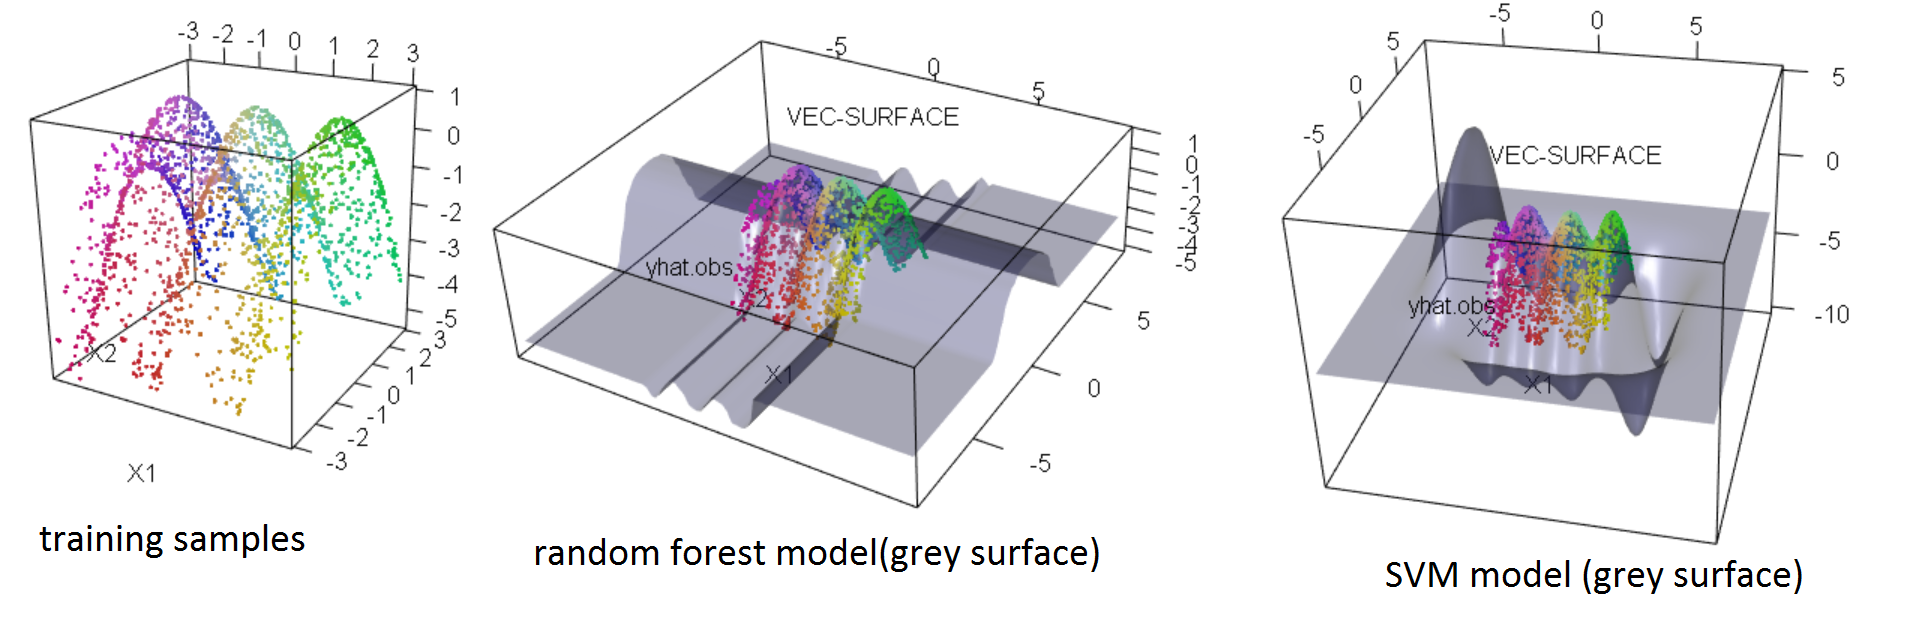
\includegraphics[width=\textwidth,height=\textheight,keepaspectratio]{graphics/svmVSrf.png}
\caption{Left plot: A training set has been simulated from  $y = sin(x1 \pi) − \frac 1 2 x_2^2$ where $x_1$ and $x_2$ are drawn from a uniform distribution within $[-3;3]$. Middle and left plot, repectively RF and RBF-SVM has been trained on the data set providing two completely similar model structures within the proximity of training data. However outside (grey surface) the RF and RBF-SVM built model structures heavily disagree. See appendix for code example.}
\label{svmVSrf}
\end{figure}


\section{random forest}
The random forest algorithm is an improvement of the classification and regression tree algorithm (CART) \cite{breiman1984classification,breiman2001random}. Overall the CART decision trees are built by applying 3 rules recursively

Rule 1: A collection of observations is called a node and a node has a prediction, the average target.

Rule 2: If a node has more than a lower limit of observations, it will be split into two nodes. A split rule is defined by a break point for given numeric features, where any observation having a feature value below or equal is forwarded to a left daughter node and otherwise to a right daughter node. Every possible split will be tried. For categorical features, any unique separation categories into to daughter nodes will be tried.

Rule 3: A loss function evaluates and select the best split, that is sum of squared residuals for regression and a variation of gini-gain for classification. See appendix for actual definition of the loss function. The regression loss function chose the split, maximize the variance across daughter nodes and minimize intra-daughter node variance. The classification loss function chose the split that produces two nodes most unlike a uniform class distribution.

Rule 4: If a node cannot be split, either as there is no valid feature left to split by or if the node do not meet the splitting criteria, the node is terminal, otherwise repeat rule 1-4 for every sub node.

Left plot of third figure of the article \textit{Forest Floor Visualizations of Random Forests} in Section \ref{sec:forestFloor} is a good example of how nodes are split and how to depict the model structure.




\subsection{Feature selection}
In order 
A crude solution is to univariatly filter any feature or interaction term, that do not have a linear relationship (e.g. pearson correlation) or have a non-linear relationship (e.g. spearman correlation) above a certain threshold. A potential problem with uni-variate feature selection 




\subsection{Feature selection}
In order 
A crude solution is to univariatly filter any feature or interaction term, that do not have a linear relationship (e.g. pearson correlation) or have a non-linear relationship (e.g. spearman correlation) above a certain threshold. A potential problem with uni-variate feature selection 


